\section{问题描述}
\label{secDynamics}

传统的多翼机的特点是具有偶数个(至少四个)大小相等的固定螺距螺旋桨,这些螺旋桨围绕几何中心以旋转对称的方式排列,几何中心大致与飞行器的电池、电子设备和有效载荷重合。 
螺旋桨手性交替排列,以便使它们的空气动力学的反应扭矩的总和为零。 

除了这种典型的配置外,许多其它的设计也是可能的,并且已经被考虑过。 
例如,使用直径大不相同的螺旋桨以提高效率 \cite{pounds2002design},使螺旋桨可倾斜 \cite{ryll2012modeling},以及螺旋桨不对齐的飞行器,使其平移能力被完全激励 \cite{mehmood2016maneuverability}。
尽管这类飞行器并不完全符合下面的描述,但它们的姿态控制问题是相似的,因为它们能够产生任意的3D扭矩,因此它们的姿态动力学是被完全激励的。
%There are, however, multicopter designs where the attitude dynamics are not fully actuated, see e.g. \cite{mueller2015relaxed,zhang2016controllable}.

\subsection{动力学}

\begin{figure}
  \centering
  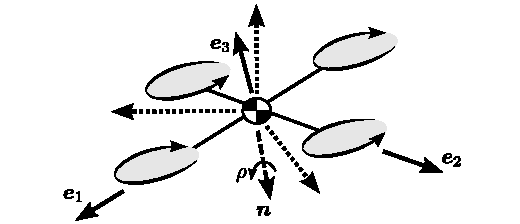
\includegraphics{Figures/quadcopter.pdf}
  \caption{
  一架多旋翼飞机带机体固连轴 $\baseVec{1}$、$\baseVec{2}$ 和 $\baseVec{3}$,从点线表示的期望的轴,被 $\rotMat$ 旋转过来。
  旋转 $\rotMat$ 是围绕单位向量 $\rotAxis$,角度为 $\rotAngle$ 的旋转。
  }
  \label{figModel}
\end{figure}

多旋翼飞机的方向(将机体固连坐标系与惯性坐标系联系起来)由旋转矩阵 $\rotMat\in\SOthree$ 描述,而角速度由 $\angVel\in\realNums^3$ 给出。 
旋转矩阵主要通过推力向量的方向来影响多旋翼飞机的运动,推力向量相对于飞行器有固定方向。

飞行器的螺旋桨都在相同的机体固连方向上产生推力 $\thrustDir$,并且量值为 $\thrustMag$,示意图参见 \figref{figModel}。
飞行器具有质量 $\mass$,受到重力加速度 $\gravity$ 的作用,因此,飞行器平移加速度 $\translAcc$ 给出为 
\begin{align}
	\translAcc = \frac{1}{\mass} \rotMat \thrustDir \thrustMag + \gravity. \label{eqDynamicsTranslAcc}
\end{align}
因此,通过控制飞行器的姿态和指定总推力,可以控制平移加速度。
从方程 \eqref{eqDynamicsTranslAcc} 中值得注意的是,姿态的三个自由度中只有两个与平移动力学有关,特别是围绕飞行器的 $\baseVec{3}$ 轴的旋转并不重要。 

姿态演变为 
\begin{align}
	\dot{\rotMat} = \rotMat \skewSym{\angVel}
\end{align}
其中 $\skewSym{\cdot}: \realNums^3\rightarrow\sothree$ 产生向量参数的倾斜对称矩阵形式 (通常称为 ``hat-map''),特别是如果 $\mvec{x}=\mrb{x_1, x_2, x_3}$ 则 
\begin{align}
	\skewSym{\mvec{x}} = \mmat{0 & -x_3 & x_2\\ x_3 & 0 & -x_1 \\ -x_2 & x_1 & 0}
\end{align}
值得注意的是,对于 $\mvec{x},\mvec{y}\in\realNums^3$ 以及 $\rotMat\in\SOthree$ \cite{bernstein2009matrix}
\begin{align}
  \skewSym{\mvec{x}} &= -\skewSym{\mvec{x}}^T
\\\skewSym{\mvec{x}}\mvec{y} &= \mvec{x}\times\mvec{y} = -\skewSym{\mvec{y}}\mvec{x}
\\\skewSym{\rotMat\mvec{x}} &= \rotMat\skewSym{\mvec{x}} \rotMat^T
\end{align}
上述 $\skewSym{\cdot}$ 的逆函数是 $\skewSymInv{\cdot}:\sothree\rightarrow\realNums^3$,所以
\begin{align}
	\skewSymInv{\skewSym{\mvec{x}}} = \mvec{x}
\end{align}

角加速度 $\angAcc$ 是飞行器质量惯性矩张量 $\mmoi$、作用在飞行器上的外部力矩 $\moments$ 和当前角速度的函数,为 
\begin{align}
	\angAcc = \dot{\angVel} = \mmoi^{-1}\mrb{\moments - \skewSym{\angVel}\mmoi\angVel} \label{eqDynamicsAngAcc}
\end{align}

所有传统多旋翼飞机(四旋翼、六旋翼和八旋翼)的配置都可以使飞行器产生一个任意(达到电机力饱和)的三维力矩 $\moments$,其与总推力 $\thrustMag$无关。
作为单个螺旋桨力的函数,力矩和总推力的计算以直截了当的方式遵循飞行器的几何形状和螺旋桨的特性。
典型的多旋翼飞机的一个重要特征是,它们能够在垂直于推力向量的方向上产生比围绕推力向量大得多的扭矩。
这是由于螺旋桨与质心的距离很大,这可能比螺旋桨的空气动力扭矩与推力的比率大一个数量级以上。 
对于敏捷机动在计算推力方面的深入讨论,示例参见文献 \cite{faessler2017thrust}。

\subsection{控制问题}
因此,从方程 \eqref{eqDynamicsAngAcc} 可以看出,在任何瞬时角速度下都可以产生任意的角加速度 $\angAcc$ (直至电机推力饱和)。
这促使将角加速度用作姿态子系统的控制输入,并且特别的是,这意味着多旋翼飞机的姿态可以被视为被完全激励,从而得到更简单的姿态动力学:
\begin{align}
	\dot{\rotMat} &= \rotMat\skewSym{\angVel}
\\	\dot{\angVel} &= \angAcc
\end{align}

我们认为控制问题是将飞行器的方向控制在一个期望的姿态 $\rotMatDes$,它有一个相关的期望的角速度 $\angVelDes$ 和角加速度 $\angAccDes$,以便 
\begin{align}
	\ddt\rotMatDes =& \rotMatDes \skewSym{\angVelDes}
\\  \ddt \angVelDes =& \angAccDes
\end{align}
旋转误差 $\rotMatErr$ 和它的角速度 $\angVelErr$ 被定义为 
\begin{align}
	\rotMatErr =& \rotMatDes^{-1} \rotMat \label{eqDefineRotMatErr}
\\  \ddt \rotMatErr =& \rotMatErr \skewSym{\angVelErr} \label{eqDefineAngVelErr}
\end{align}

代入旋转误差的定义,并经过一些代数运算,由此得出 
\begin{align}
  \angVelErr &= \angVel - \rotMatErr^{-1} \angVelDes
\\ \angAccErr &= \ddt \angVelErr = \angAcc - \rotMatErr^{-1} \angAccDes + \skewSym{\angVelErr} \angVelDes \label{eqDefAngAccErr}
\end{align}

为紧凑起见,我们将使用 $\angAccErr$ 作为控制输入,注意,指令扭矩是通过将方程 \eqref{eqDefAngAccErr} 代入方程 \eqref{eqDynamicsAngAcc} 恢复的。

为了进行分析,通常更直观的方法是将旋转矩阵 $\rotMat$ 表示为旋转向量,其被分解为角度 $\rotAngle\in[0,\pi]$ 和单位长度旋转轴 $\rotAxis$ (通常称为特征轴)。
这些数量之间的关系由文献 \cite{shuster1993survey} 给出为 
\begin{align}
	\rotMat = \cos\rotAngle\identityMat + \mrb{1-\cos\rotAngle}\rotAxis\rotAxis^T + \sin\rotAngle\skewSym{\rotAxis}
	\label{eqRotMatFromAxisAngle}
\end{align}
由此,给定旋转矩阵的角度和轴也可以直接向前恢复,除非以 $180^\circ$ 的旋转,此时围绕 $\rotAxis$ 和 $-\rotAxis$ 的旋转是相同的,以及与轴不相关的零旋转。







